\chapter{Part 1: Business Requirements}


\section{Background}
Even for the most relaxed students, university may be challenging. For many, this is the first time that you live away from family, friends and home comforts, but there are things you can do to keep your worries at bay.Stress is a normal part of life to some extent, it is only when the amount we experience exceeds our ability and resources to manage it that we find ourselves in a vicious stress cycle.Stress is the body's physical and mental response to its demands. It is the result of our response to events outside, not necessarily the events themselves.Students are always looking for a way to relieve stress through different ways.
 
\section{Business Opportunity}
The rise of stress in the work place has given us a large business opportunity to help those in need of stress reduction.Creating a game for stress relief seems like a fantastic business opportunity. Studies have also shown that action-based video games not only reduce stress but can also sharpen cognitive skills such as speed of reaction. This can help gamers think faster on their feet and are likely to be better able to solve problems, which can also \href{https://www.verywellmind.com/active-problem-solving-425384}{reduce stress} in other ways. 

\section{Business Objectives}
\begin{center}

 \begin{tabular}{ l p {10cm}}
 
 \hline
  Objective & Description \\ [0.5ex] 
 \hline\hline
 1 & Reduce the stress students feel within 1 month of playing the game \\ 
 \hline
 2 & Help students improve their skills in every day life \\
 \hline
 3 & Help students achieve more by reducing their stress

\end{tabular}

\end{center}
\section{Success Metrics}

\begin{center}

 \begin{tabular}{ l p {10cm}}
 
 \hline
  Success Metric & Description \\ [0.5ex] 
 \hline\hline
 1 & Decrease the stress levels of students by 75\% in 3 months \\ 
 \hline
 2 & People download the game more than 1000 times in 1 month from the company website \\
 \hline
 3 & Create a community of players around the game from the day of release

\end{tabular}

\end{center}

\section{Vision Statement}
For students who wish to reduce their stress from every day life "Adventures of Vman" is a game where the player kills enemies that them using the power of fire.The players will navigate through the level trying to avoid or kill enemies and will ultimately be met with a huge enemy boss which they will have to beat to be able to beat the game. The game aims to transfer the player into a stress free world were they can release all their stress.
\section{Business Risks}

\begin{center}

 \begin{tabular}{ l p {10cm}}
 
 \hline
  Risk & Description \\ [0.5ex] 
 \hline\hline
 1 & The game might not be a big hit with players thus exposure will be low. \\ 
 \hline
 2 & Students that are stressed might prefer non-action games instead \\
 \hline
 3 & The game might have a negative effect instead of a positive effect to some players and might induce stress instead.

\end{tabular}

\end{center}
\section{Business Assumptions and Dependencies}
\subsection{Business assumptions}
\begin{enumerate}
	\item User has access to the internet to download the game
	\item User has a laptop or Desktop computer running Windows/Mac Os/Linux
	\item We assume the server hosting the game will be available at all times
	\item There are people willing to play the game
	\item Users have a basic knowledge of installing and running games on their computer
\end{enumerate}

\subsection{Dependencies}
The game will depend upon the players comprehension of how the game works and is up to the player understand the mechanics of the game. The game depends on the system that it will run on, if its too slow it might not be optimal to run the game.

\chapter{Part 2: Scope and Limitations}


\section{Major Features}
\begin{itemize}
    \item Jumping
    A necessary mechanic of the game which allow sudden movements when trying to avoid enemies , cross obstacles or attack enemies which are higher up.
    \item Attack
    The fundamental mechanic to beating the game as it requires the player to kill enemies to reach the end boss. The attack mechanic fires "balls of fire" which deal damage to enemies.
    \item Crouch
    The player can crouch so he can get through tight places it also slows the player down which can help in moving more precisely.
\end{itemize}
\section{Scope of initial release}
\begin{center}

 \begin{tabular}{ l p {10cm}}
 
 \hline
  Feature & Description \\ [0.5ex] 
 \hline\hline
 1 & The player can jump with a constant force but cannot double jump while in the air. \\ 
 \hline
 2 & The attack function will deal constant damage and will not increase with power ups for now \\
 \hline
 3 & The game will have parts where slowing down and crouching with help the player move around and attack enemies.

\end{tabular}
\end{center}

\section{Limitations and Exclusions}
\begin{enumerate}
	\item The game is limited to using Unity2D
	\item The game is designed to run on Desktop operating systems.
	\item We cant make the game to hard as it will stress the players out.
\end{enumerate}

\chapter{Business Context}

\section{Stakeholder Profiles}
\begin{figure}[hbt!]
    \centering
    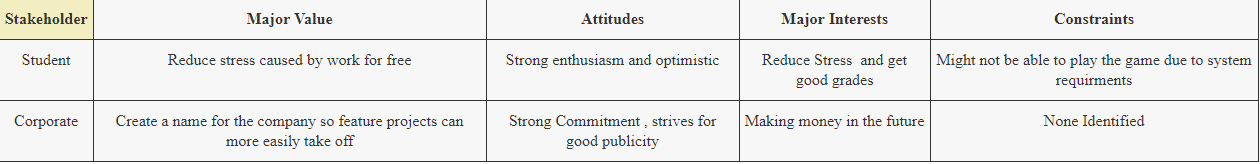
\includegraphics[width=167mm,scale=1]{images/table.png}
    \caption{Stake holders}
    \label{fig:diagram}
\end{figure}

\subsection{Project Profiles}

\section{Deployment Consideration}



